% https://tex.stackexchange.com/questions/16232/how-to-plot-fx-sinx-kx-cosx-and-ux-x%C2%B2-with-tikz
\documentclass{article}
\usepackage{pgfplots}

\begin{document}
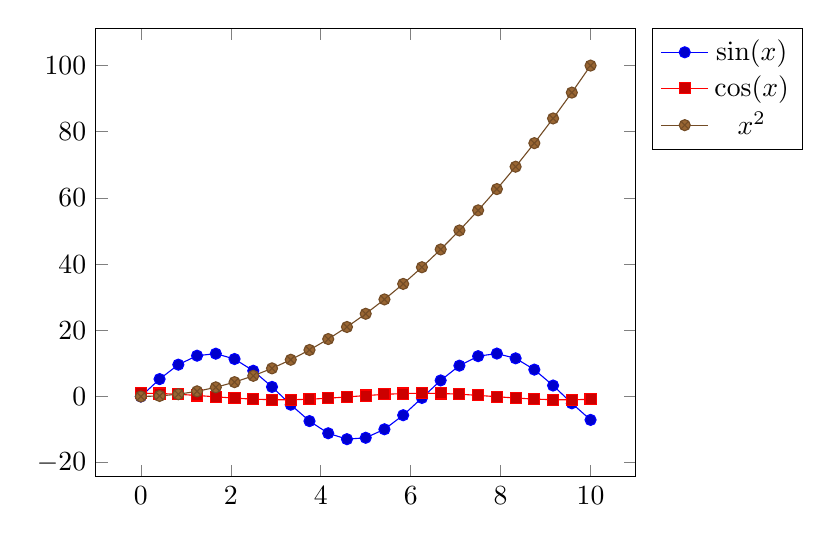
\begin{tikzpicture}
    \begin{axis}[domain=0:10,legend pos=outer north east]
    \addplot {13*sin(deg(x))}; 
    \addplot {cos(deg(x))}; 
    \addplot {x^2};
    \legend{$\sin(x)$,$\cos(x)$,$x^2$}
    \end{axis}
\end{tikzpicture}
\end{document}